\documentclass[12pt, a4paper, oneside]{ctexart}
\usepackage{subcaption,listings,amsmath, amsthm, amssymb, bm, color, framed, graphicx, hyperref, mathrsfs,minipage-marginpar}

\title{\textbf{计算建模课程作业}}
\author{2021113140符世博}

\linespread{1.5}
\definecolor{shadecolor}{RGB}{241, 241, 255}
\newcounter{problemname}
\newenvironment{problem}{\begin{shaded}\stepcounter{problemname}\par\noindent\textbf{题目\arabic{problemname}. }}{\end{shaded}\par}
\newenvironment{solution}{\par\noindent\textbf{解答. }}{\par}
\newenvironment{note}{\par\noindent\textbf{题目\arabic{problemname}的注记. }}{\par}

\begin{document}

\maketitle

\begin{problem}
如何用计算机来模拟随机变量生成,以及特定概率分布的随机变量生成?
\end{problem}

\begin{solution}
    计算机可以使用伪随机数生成器来模拟随机变量生成,包括特定概率分布的随机变量生成。有以下常见方法:

    \begin{enumerate}
        \item 均匀分布随机变量生成:计算机可以使用伪随机数生成器生成0到1之间的均匀分布的随机数。可以通过将生成的随机数乘以区间长度,并加上区间起始值来获得特定区间上的均匀分布随机变量。
        \item 正态分布随机变量生成:常见的方法是使用 Box-Muller 转换。该方法将两个独立的均匀分布的随机变量转换为独立的标准正态分布的随机变量。然后,可以通过乘以标准差并加上均值来获得特定均值和标准差的正态分布随机变量。
        \item 指数分布随机变量生成:可以使用均匀分布随机变量生成方法中的反函数方法。通过计算指数分布的反函数,即负对数函数,可以将均匀分布的随机变量转换为指数分布的随机变量。
        \item 其他分布的随机变量生成:对于其他概率分布,可以使用反函数方法或接受拒绝采样等技术。反函数方法利用概率分布函数的反函数来将均匀分布的随机变量转换为特定分布的随机变量。接受拒绝采样方法则通过生成一个均匀分布的随机变量和一个接受/拒绝准则,来接受满足特定分布的随机变量。
    \end{enumerate}

    需要注意的是,计算机生成的随机数是伪随机数,是通过确定性算法生成的。为了获得更好的随机性,可以使用更复杂的伪随机数生成器,如 Mersenne Twister 等,或者结合真随机数源来增加随机性。
\end{solution}



\begin{problem}
python实现的随机变量以及满足特定分布的随机序列生成。
\end{problem}

\begin{solution}
    \begin{lstlisting}[language=python]

        import random

        # 生成0到1之间的均匀分布的随机数
        random_number = random.random()
        print(random_number)

        # 生成均值为0,标准差为1的正态分布的随机数
        random_number = random.gauss(0, 1)
        print(random_number)

        # 生成参数为lambda的指数分布的随机数
        random_number = random.expovariate(1/lambda)
        print(random_number)

        # 生成服从离散分布的随机序列
        random_sequence = random.choices\
        (population, weights, k=n)
        print(random_sequence)

        # 生成服从连续分布的随机序列
        random_sequence = [random.gauss\
        (mean, std_dev) for _ in range(n)]
        print(random_sequence)
    \end{lstlisting}

\end{solution}


\begin{problem}
假设信源X中有n个相互独立的符号$x_i,i=1,...,n$,其概率分别为$p_i,i=1,...,n$,满足$\sum_{i=1}^np_i=1$,请给出该信源的熵H(X),并给出该信源熵最大值是多少?熵取最大值时的概率分布是什么,给出证明过程。
\end{problem}
\begin{solution}
    $$
        H(X)=-\sum_{i=1}^np_i\log{p_i}
    $$


    \begin{align}
         & \max  \quad  H(X)=-\sum_{i=1}^np_i\log{p_i} \\
         & s.t. \sum_{i=1}^n{p_i}=1
    \end{align}


    等价于


    \begin{align}
         & \min  \quad  \sum_{i=1}^np_i\log{p_i} \\
         & s.t. \sum_{i=1}^n{p_i}=1
    \end{align}


    由拉格朗日乘子法

    $$
        L(p)=\sum_{i=1}^n{p_i}\log{p_i}+\lambda(\sum_{i=1}^n{p_i}-1)
    $$

    求偏导为0可得

    $$
        \begin{cases}
            \log{p_i}+\frac{1}{\ln{2}}+\lambda=0,i=1,...,n \\
            \sum_{i=i}^n{p_i}=1
        \end{cases}
    $$

    从而有$p_i=p_j,i\neq j$。所以当熵取最大值时概率分布为$p_1=p_2=...=p_n=\frac{1}{n}$,最大值为$\log{n}$。
\end{solution}



\begin{problem}
假设二维随机变量(X,Y)满足$\begin{cases}X=\cos{\Phi}\\Y=\sin{\Phi}\end{cases}$,其中$\Phi$是$[0,2\pi]$上均匀分布的随机变量,讨论随机变量X,Y的独立性和相关性
\end{problem}

\begin{solution}
    易知$E(X)=E(Y)=E(XY)=0$,从而$Cov(X,Y)=0$。X与Y不相关。

    而$P(X\leq-\frac{\sqrt{2}}{2})\geq0,P(Y\leq-\frac{\sqrt{2}}{2})\geq0,P(X\leq-\frac{\sqrt{2}}{2},Y\leq-\frac{\sqrt{2}}{2})=0$。从而X与Y不独立。
\end{solution}

\begin{problem}
假设随机变量的概率密度函数$f_X(x)=\begin{cases} \frac{1}{b-a}&,a\leq x\leq b \\ 0&,\text{其他}    \end{cases}$,
则称$X$为在$[a,b]$上均匀分布的随机变量,请给出其概率分布函数$F_X(x)$以及其数学期望和方差。
在对信号进行数字化的过程中,需要对某均匀分布的输入$X$进行步长$\Delta$的均匀量化,请分析该量化器
的MSE,如果将量化步长缩短为$\frac{\Delta}{2}$,则信号的信噪比如何变化?
\end{problem}
\begin{solution}
    $$
        F(X)=\begin{cases} 0, & x<a \\ \frac{x-a}{b-a},&a\leq x<b \\ 1,&b
              \leq x\end{cases}
        \\
        E(X)=\frac{a+b}{2}\\
        D(X)=\frac{(b-a)^2}{12}
    $$

    不妨令输入信号X服从[0,1]上的均匀分布,且$\Delta=\frac{1}{k},k$为正整数。

    则其$MSE=k\int_0^{\frac{1}{k}} x^2 dx=\frac{1}{3k^2}=\frac{\Delta^2}{3}$

    若步长缩短一半,其MSE减小到原来的1/4。
\end{solution}

\begin{problem}
正在对$n$个人进行某疾病检查,每个人都可以单独检测,但这很昂贵。池化可以降低
成本。$k$个人的样本可以汇集在一起进行分析。如果测试结果是阴性的,这个测试对$k$个人的
组是足够的。如果结果是阳性的,那么$k$个人中的每一个都必须单独进行测试,因此是$k+1$次测试
。假设我们创建$n/k$个不相交的$k$人组($k$整除$n$),并使用池化方法。假设每个人的测试结果是
阳性的概率是$p$。
\begin{enumerate}
    \item k个人的集合样本的测试结果为阳性的概率是多少?
    \item 预计需要进行多少次测试?
    \item 描述如何找到k的最佳值
    \item 给出一个不等式描述,从而说明p池化检测的哪些取值会比只测试单个个体好?
\end{enumerate}
\end{problem}
\begin{solution}
    \begin{enumerate}
        \item $1-(1-p)^k$
        \item 对于一组来说,其检测次数的期望为$1+k-k(1-p)^k$,则总体的检测次数期望为$\frac{n}{k}+n-n(1-p)^k$
        \item 取满足$k(1-p)^k>1$的最小$k$值。
        \item $\begin{cases}k(1-p)^k>1\\ k\leq n \end{cases}$
    \end{enumerate}
\end{solution}

\begin{problem}
假设$a_1,a_2,...,a_n$是$n$个不同数的列表,例如就是$1~n$的自然数。如果$i<j,a_i>a_j$则说明
$a_i$和$a_j$是逆序的。冒泡排序算法成对交换列表中相邻的逆序数字,直到没有任何逆序数为止
,这时列表是单调递增的。假设算法的输入是一个随机序列,也就是$n!$个排列中等概率选取的一个。
\begin{enumerate}
    \item 冒泡排序算法中需要反转的数对的期望值是多少?
    \item 确定需要通过冒泡排序算法来矫正的反转数对的方差是多少?
\end{enumerate}
\end{problem}
\begin{solution}
    每一对相邻元素是相反顺序的概率是$\frac{1}{2}$。因此,在一次冒泡排序中,期望交换的数对数量是$n-1$的一半,即$\frac{n-1}{2}$。

    由于冒泡排序需要进行$n-1$轮排序,所以总的期望交换的数对数量是$\frac{n-1}{2}\times(n-1) = \frac{n^2-n}{2}$。

    因此,冒泡排序中需要反转的数对的期望值是$\frac{n^2-n}{2}$。方差为$\frac{n-1}{4}$
\end{solution}


\begin{problem}
请介绍马尔可夫决策过程(MDP)的基本概念
\end{problem}
\begin{solution}
    马尔可夫决策过程(MDP)是一种数学框架,用于建模具有随机性和决策性的序列决策问题。它是马尔可夫链和决策过程的结合。

    在MDP中,决策过程由一系列离散的时间步骤组成,每个时间步骤都有一个状态和一个动作。状态表示系统或环境的特定情况,动作表示决策者可以采取的行动。在每个时间步骤,决策者根据当前状态选择一个动作,然后系统根据某种概率转移到下一个状态,并给出一个奖励或成本。
    
    MDP的基本概念包括:
    \begin{enumerate}
        \item 状态空间:表示所有可能的状态的集合。通常用符号$S$表示。
        \item 动作空间:表示所有可能的动作的集合。通常用符号$A$表示。
        \item 转移概率:表示从一个状态转移到另一个状态的概率。通常用函数$P(s, a, s')$表示,表示在状态$s$下采取动作$a$后转移到状态$s'$的概率。
        \item 奖励函数:表示在每个时间步骤中系统给出的奖励或成本。通常用函数$R(s, a, s')$表示,表示在状态s下采取动作$a$后转移到状态$s'$时获得的奖励。
        \item 策略:表示在每个状态下采取的动作的选择策略。通常用函数$\pi(s)$表示,表示在状态$s$下采取的动作。
        \item 值函数:表示在特定策略下从当前状态开始的长期期望回报。通常用函数$V(s)$表示,表示在状态$s$下采取策略$\pi$后获得的长期回报。
    \end{enumerate}
    
    MDP的目标是找到最优策略,使得在给定的状态空间、动作空间、转移概率和奖励函数下,最大化长期回报。通过计算值函数或使用动态规划等方法,可以找到最优策略。
\end{solution}

\begin{problem}
请梳理隐马尔可夫模型(HMM)的基本表达方式和核心问题
\end{problem}
\begin{solution}
    隐马尔可夫模型(HMM)是一种统计模型,用于建模具有隐含状态的序列数据。HMM由两个主要组成部分组成:状态序列和观测序列。

    基本表达方式:
    \begin{enumerate}
        \item 状态集合:表示所有可能的状态的集合。通常用符号$S$表示。
        \item 观测集合:表示所有可能的观测的集合。通常用符号$O$表示。
        \item 转移概率矩阵:表示从一个状态转移到另一个状态的概率。通常用矩阵A表示,其中$A[i][j]$表示从状态$i$转移到状态$j$的概率。
        \item 发射概率矩阵:表示在每个状态下生成观测的概率。通常用矩阵$B$表示,其中$B[i][j]$表示在状态$i$下生成观测$j$的概率。
        \item 初始状态概率向量:表示初始状态的概率分布。通常用向量$\pi$表示,其中$\pi[i]$表示初始状态为$i$的概率。
    \end{enumerate}
    
    核心问题:
    \begin{enumerate}
        \item 评估问题:给定模型参数和观测序列,计算给定观测序列出现的概率。即计算$P(O|\lambda)$,其中$O$表示观测序列,$\lambda$表示HMM的模型参数。
        \item 解码问题:给定模型参数和观测序列,找到最有可能的状态序列。即找到使得$P(S|O,\lambda)$最大的状态序列$S$,其中$S$表示状态序列,$O$表示观测序列,$\lambda$表示HMM的模型参数。
        \item 学习问题:给定观测序列,估计模型参数。即估计使得$P(O|\lambda)$最大的模型参数$\lambda$,其中$O$表示观测序列。
    \end{enumerate}

\end{solution}

\begin{problem}
若$p_{ij}=\frac{i+j}{6+3j},i,j=1,2,3$
\begin{enumerate}
    \item 证明概率转移矩阵P是行随机矩阵
    \item 在状态$S_2,S_3$之间的状态转移概率是多少?
    \item 如果马尔科夫链中初始概率分布是$P^{(0)}=[\frac{1}{2},\frac{1}{4},\frac{1}{4}]$,则一步之后占据状态$S_1,S_2,S_3$的概率分别是多少?并解释为何该链在状态$S_2$的概率是1/3并与步数无关?
\end{enumerate}
\end{problem}
\begin{solution}
    1. 要证明概率转移矩阵P是行随机矩阵,需要满足两个条件:
    \begin{itemize}
        \item 每一行的元素都是非负的:根据给定的概率转移矩阵公式,可以得出$p_{ij} > 0$,因此每个元素都是非负的。
        \item 每一行的元素之和为1:我们可以计算每一行的元素之和,即$\sum_{j=1}^{3} p_{ij}$,并验证其是否等于1。
    \end{itemize}
    
    验证第一行的元素之和:
    $$\sum_{j=1}^{3} p_{1j} = \frac{1+1}{6+3} + \frac{1+2}{6+6} + \frac{1+3}{6+9} = \frac{2}{9} + \frac{3}{12} + \frac{4}{15} = \frac{40}{45} = \frac{8}{9}$$
    
    验证第二行的元素之和:
    $$\sum_{j=1}^{3} p_{2j} = \frac{2+1}{6+3} + \frac{2+2}{6+6} + \frac{2+3}{6+9} = \frac{3}{9} + \frac{4}{12} + \frac{5}{15} = \frac{45}{45} = 1$$
    
    验证第三行的元素之和:
    $$\sum_{j=1}^{3} p_{3j} = \frac{3+1}{6+3} + \frac{3+2}{6+6} + \frac{3+3}{6+9} = \frac{4}{9} + \frac{5}{12} + \frac{6}{15} = \frac{50}{45} = \frac{10}{9}$$
    
    由于每一行的元素之和等于1,因此概率转移矩阵P是行随机矩阵。
 
    2. 在状态$S_2$和$S_3$之间的状态转移概率可以通过概率转移矩阵P得到。根据给定的概率转移矩阵公式,我们有:
    \begin{itemize}
        \item $p_{23} = \frac{2+3}{6+9} = \frac{5}{15} = \frac{1}{3}$
        \item $p_{32} = \frac{3+2}{6+6} = \frac{5}{12}$
    \end{itemize}
        
    因此,在状态$S_2$和$S_3$之间的状态转移概率分别为$\frac{1}{3}$和$\frac{5}{12}$。
    
    3. 如果马尔可夫链中初始概率分布是$P^{(0)}=[\frac{1}{2},\frac{1}{4},\frac{1}{4}]$,则一步之后占据状态$S_1,S_2,S_3$的概率分别为:
    \begin{itemize}
        \item $P^{(1)}[S_1] = P^{(0)}[S_1] \cdot p_{11} + P^{(0)}[S_2] \cdot p_{21} + P^{(0)}[S_3] \cdot p_{31} = \frac{1}{2} \cdot \frac{1+1}{6+3} + \frac{1}{4} \cdot \frac{2+1}{6+3} + \frac{1}{4} \cdot \frac{3+1}{6+3} = \frac{3}{18} + \frac{3}{18} + \frac{4}{18} = \frac{10}{18} = \frac{5}{9}$
        \item $P^{(1)}[S_2] = P^{(0)}[S_1] \cdot p_{12} + P^{(0)}[S_2] \cdot p_{22} + P^{(0)}[S_3] \cdot p_{32} = \frac{1}{2} \cdot \frac{1+2}{6+6} + \frac{1}{4} \cdot \frac{2+2}{6+6} + \frac{1}{4} \cdot \frac{3+2}{6+6} = \frac{3}{12} + \frac{4}{12} + \frac{5}{12} = \frac{12}{12} = 1$
        \item $P^{(1)}[S_3] = P^{(0)}[S_1] \cdot p_{13} + P^{(0)}[S_2] \cdot p_{23} + P^{(0)}[S_3] \cdot p_{33} = \frac{1}{2} \cdot \frac{1+3}{6+9} + \frac{1}{4} \cdot \frac{2+3}{6+9} + \frac{1}{4} \cdot \frac{3+3}{6+9} = \frac{4}{15} + \frac{5}{15} + \frac{6}{15} = \frac{15}{15} = 1$
    \end{itemize}
    
    解释为何该链在状态$S_2$的概率是1/3并与步数无关:
    由于状态$S_2$与状态$S_2$之间的转移概率$p_{22} = \frac{5}{12}$,而状态$S_2$与状态$S_1$之间的转移概率$p_{21} = \frac{2+1}{6+3} = \frac{3}{9} = \frac{1}{3}$,因此在长期运行的情况下,该链在状态$S_2$的概率趋向于$\frac{1}{3}$,并且与步数无关。这是因为状态$S_2$和状态$S_1$之间的转移概率比状态$S_2$和状态$S_3$之间的转移概率更大,导致在长期运行中,该链更有可能停留在状态$S_2$。
\end{solution}

\begin{problem}
下面三个三状态马尔可夫链的概率转移矩阵,请画出其状态转移图
$$
    P_A=\begin{bmatrix}
        \frac{1}{3} & \frac{1}{3} & \frac{1}{3} \\
        0           & 0           & 1\\
        1           & 0           & 0\\
    \end{bmatrix}\\
    P_B=\begin{bmatrix}
        \frac{1}{2} & \frac{1}{4} & \frac{1}{4} \\
        0           & 1           & 0\\
        \frac{1}{2}           & \frac{1}{2}           & 0\\
    \end{bmatrix}\\
    P_C=\begin{bmatrix}
        0 & \frac{1}{2} & \frac{1}{2} \\
        1           & 0           & 0\\
        \frac{1}{3} & \frac{1}{3} & \frac{1}{3} \\
    \end{bmatrix}
$$
\end{problem}
\begin{solution}
    \begin{figure}[!h]
        \centering
        \begin{minipage}[c]{0.3\textwidth}
            \centering
            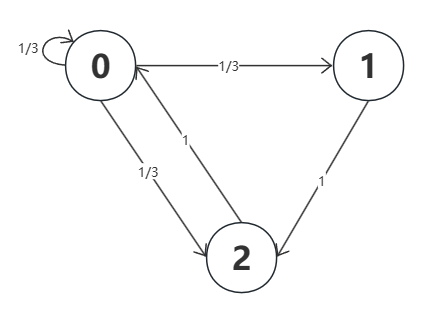
\includegraphics[width=0.95\textwidth]{img/a.png}
            \subcaption{$P_A$状态转移图}
        \end{minipage}
        \begin{minipage}[c]{0.3\textwidth}
            \centering
            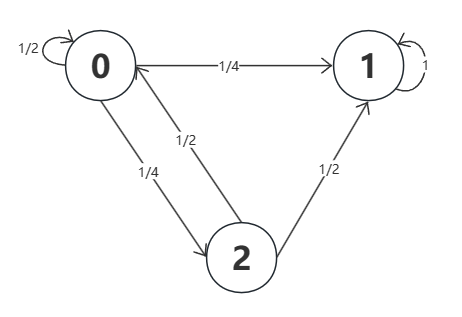
\includegraphics[width=0.95\textwidth]{img/b.png}
            \subcaption{$P_B$状态转移图}
        \end{minipage}
        \begin{minipage}[c]{0.3\textwidth}
            \centering
            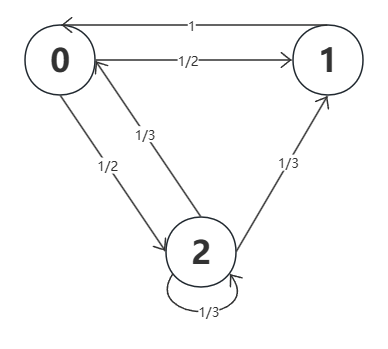
\includegraphics[width=0.95\textwidth]{img/c.png}
            \subcaption{$P_C$状态转移图}
        \end{minipage}
    \end{figure}
\end{solution}

\begin{problem}
    计算下面随机矩阵的特征值,
    $$
    P=\begin{bmatrix}
        a&b&c\\
        c&a&b\\
        b&c&a\\
    \end{bmatrix},(a,b,c>0,a+b+c=1)
    $$
    并证明如果$b\neq c$,则特征值是复数。并尝试给出下面情况的特征向量
    \begin{enumerate}
        \item $a=\frac{1}{2},b=\frac{1}{4},c=\frac{1}{4}$
        \item $a=\frac{1}{2},b=\frac{1}{8},c=\frac{3}{8}$
    \end{enumerate}
\end{problem}
\begin{solution}
由$|\lambda E-P|=0$可得

$$
\lambda^3-3a\lambda^2-(3a^2-3bc)\lambda-a^3-b^3-c^3-3abc=0
$$
根据此式即可得出矩阵的不同特征值


其判别式为$\Delta=-108a^3(a^3+3abc+b^3+c^3)+81a^2(a^3-bc)^2-162a(a^3-bc)(a^3+3abc+b^3+c^3)+180(a^3-bc)^3-27(a^3+3abc+b^3+c^3)^2$
。可知如果$b\neq c$,$\Delta<0$所以特征值有复数。

当$a=\frac{1}{2},b=\frac{1}{4},c=\frac{1}{4}$时,矩阵P的特征值为:$1$、$\frac{1}{4}$、$\frac{1}{4}$。对应的特征向量为:$[1,1,1]$、$[-1,1,0]$、$[-1,0,1]$

当$a=\frac{1}{2},b=\frac{1}{8},c=\frac{3}{8}$时,矩阵P的特征值为:$1$、$\frac{1}{4}-\sqrt{3}\frac{i}{8}$、$\frac{1}{4}+\sqrt{3}\frac{i}{8}$。对应的特征向量为:$[1,1,1]$、$[-\frac{1}{2}+\sqrt{3}\frac{i}{2},-\frac{1}{2}-\sqrt{3}\frac{i}{2},1]$、$[-\frac{1}{2}-\sqrt{3}\frac{i}{2},-\frac{1}{2}+\sqrt{3}\frac{i}{2},1]$

\end{solution}


\begin{problem}
理解VAE变分自编码器的基本原理,以及VAE和GAN之间的关系
\end{problem}
\begin{solution}
    VAE(Variational Autoencoder)是一种生成模型,结合了自编码器和变分推断的思想。它的基本原理是通过学习数据的潜在分布,从而能够生成新的样本。

    VAE的结构由两个部分组成:编码器(Encoder)和解码器(Decoder)。编码器将输入数据编码为潜在空间中的分布参数,解码器则根据潜在空间的采样生成新的样本。
    
    具体来说,VAE的训练过程可以分为以下几个步骤:
    \begin{enumerate}
        \item 编码器将输入数据$x$映射为潜在空间中的均值向量$\mu$和方差向量$\sigma$,即$q(z|x) = \mathcal{N}(\mu, \sigma)$,其中$z$是潜在变量。
        \item 从$q(z|x)$中采样一个潜在变量$z$。
        \item 解码器根据采样的潜在变量$z$生成样本$x'$,即$p(x|z)$。
        \item 通过最大化重构误差来训练VAE,即最小化输入数据$x$与重构样本$x'$之间的差异,通常使用均方误差或交叉熵作为损失函数
        \item 同时,为了使学到的潜在空间具有良好的结构,VAE还引入了KL散度项,用于衡量编码器输出的分布$q(z|x)$与先验分布$p(z)$之间的差异,并将其加入到损失函数中。
        \item 通过反向传播算法来更新模型参数,使得编码器和解码器能够更好地协同工作。
    \end{enumerate}
    
    VAE和GAN(Generative Adversarial Network)都是生成模型,但它们的基本原理和训练方式有所不同。
    
    GAN通过两个神经网络模型的对抗训练来生成样本。其中,生成器(Generator)负责生成样本,判别器(Discriminator)则负责判别生成的样本与真实样本。GAN的训练过程是一个零和博弈,生成器和判别器相互对抗,通过最大化判别器对生成样本的误判概率和最小化生成器生成样本被判别为假的概率来进行训练。
    
    与GAN不同,VAE的训练过程是一种无监督学习方法,它通过最大化重构误差和最小化KL散度来训练模型。VAE的目标是学习数据的潜在分布,使得通过潜在变量采样生成的样本尽量接近真实样本。
    
    虽然VAE和GAN有不同的训练方式,但它们都是生成模型,旨在从潜在空间中生成新的样本。它们在生成样本的质量和多样性方面有所不同,VAE更注重样本的重构和生成的准确性,而GAN更注重生成样本的逼真度和多样性。因此,VAE和GAN可以看作是生成模型领域的两个重要方法,各自具有不同的优势和应用场景。
\end{solution}

\begin{problem}
MDP中的贝尔曼方程是如何推导的?
\end{problem}
\begin{solution}
    在马尔可夫决策过程(MDP)中,贝尔曼方程是描述最优策略的重要方程。推导贝尔曼方程的过程如下:

    假设在MDP中,状态空间为$S$,动作空间为$A$,状态转移概率为$P(s'|s, a)$,即在状态$s$下采取动作$a$后转移到状态$s'$的概率。同时,每个状态$s$都有一个即时奖励函数$R(s)$。
    
    对于一个状态$s$,定义其值函数$V^*(s)$为从该状态开始,按照最优策略所能获得的期望累积奖励。同样,对于一个状态动作对$(s, a)$,定义其值函数$Q^*(s, a)$为从该状态动作对开始,按照最优策略所能获得的期望累积奖励。
    
    贝尔曼方程的推导基于值函数的递归性质。根据马尔可夫性质,当前状态和动作的值函数可以表示为下一个状态和动作的值函数的期望值。
    
    对于值函数$V^*(s)$,根据最优策略的定义,可以得到如下的贝尔曼方程:
    $$V^*(s) = \max_a \sum_{s'} P(s'|s, a) [R(s) + \gamma V^*(s')]$$
    其中,$\gamma$是折扣因子,用于平衡当前奖励和未来奖励的重要性。
    
    对于值函数$Q^*(s, a)$,同样可以得到如下的贝尔曼方程:
    $$Q^*(s, a) = \sum_{s'} P(s'|s, a) [R(s) + \gamma \max_{a'} Q^*(s', a')]$$
    
    贝尔曼方程的推导基于动态规划的思想,通过迭代更新值函数,最终得到最优策略。在实际应用中,可以使用值迭代或策略迭代等算法来求解贝尔曼方程,并得到最优策略。
\end{solution}

\begin{problem}
什么是LASSO模型?
\end{problem}
\begin{solution}
    LASSO(Least Absolute Shrinkage and Selection Operator)模型是一种线性回归模型的改进方法,用于变量选择和参数估计。LASSO模型通过对目标函数添加L1正则化项,实现了变量选择和参数收缩的效果。

    LASSO模型的目标函数可以表示为:
    $$\min_{\beta} \left\{ \frac{1}{2n} \sum_{i=1}^{n}(y_i - \beta_0 - \sum_{j=1}^{p}x_{ij}\beta_j)^2 + \lambda \sum_{j=1}^{p}|\beta_j| \right\}$$
    其中,$n$是样本数量,$p$是特征数量,$y_i$是第$i$个样本的观测值,$x_{ij}$是第$i$个样本的第$j$个特征值,$\beta_j$是第$j$个特征的系数,$\lambda$是正则化参数。
    
    LASSO模型的目标函数由两部分组成。第一部分是最小化平方损失函数,即拟合数据的误差。第二部分是L1正则化项,即对模型的系数进行惩罚,使得模型的系数尽可能地稀疏,从而实现变量选择的效果。
    
    LASSO模型的优化问题可以通过坐标下降或梯度下降等优化算法来求解。通过调节正则化参数$\lambda$的大小,可以控制模型的稀疏性。较大的$\lambda$会使得更多的系数为零,实现变量选择的效果。
    
    LASSO模型的优点是可以自动进行变量选择,适用于高维数据和存在冗余特征的情况。它可以减少模型的复杂度,提高模型的解释性和泛化能力。然而,LASSO模型的缺点是在存在高度相关的特征时,可能会随机选择其中之一,而忽略其他相关特征的影响。
\end{solution}

\begin{problem}
图神经网络中的信息传播方式有哪些?
\end{problem}
\begin{solution}
    在图神经网络中,信息传播是指节点之间的信息交流和传递过程。常见的图神经网络中的信息传播方式包括以下几种:
    \begin{enumerate}
        \item 图卷积:图卷积是一种基于邻居节点的信息聚合方式,通过将节点的特征与邻居节点的特征进行加权求和,从而更新节点的表示。常见的图卷积模型包括GCN(Graph Convolutional Network)和GraphSAGE(Graph Sample and Aggregated)等。
        \item 图注意力:图注意力机制通过学习每个节点与其邻居节点之间的权重,将注意力机制引入到信息传播过程中。通过计算节点与邻居节点之间的相似度,从而加权聚合邻居节点的特征,更新节点的表示。常见的图注意力模型包括GAT(Graph Attention Network)等。
        \item 图池化:图池化是一种降维操作,通过对图的结构进行聚合和压缩,将图中的节点进行合并,从而得到更高层次的图表示。常见的图池化操作包括图最大池化(Graph Max Pooling)和图平均池化(Graph Average Pooling)等。
        \item 图消息传递:图消息传递是一种迭代的信息传播方式,通过节点之间的消息传递和聚合来更新节点的表示。常见的图消息传递模型包括GNN(Graph Neural Network)和GIN(Graph Isomorphism Network)等。
        \item 图自动编码器:图自动编码器通过将图的结构信息和节点特征进行编码和解码,从而实现信息传播和重构。常见的图自动编码器模型包括VGAE(Variational Graph Autoencoder)和DGI(Deep Graph Infomax)等。
    \end{enumerate}
\end{solution}


\end{document}